\documentclass[preview=true]{standalone}
\usepackage{tikz}
\usepackage{pgfplots}
\usepackage[siunitx, american]{circuitikz}
\usepackage[utf8]{inputenc}
\usepackage{newtxtext,newtxmath}
\usepackage[T1]{fontenc}
\pgfplotsset{compat=1.18}
\usepgfplotslibrary{units, fillbetween, smithchart, colormaps}
\usetikzlibrary{positioning, shapes, arrows, arrows.meta, graphs, shapes.geometric, math}
\tikzset{>=latex} % Better arrow tips

\begin{document}
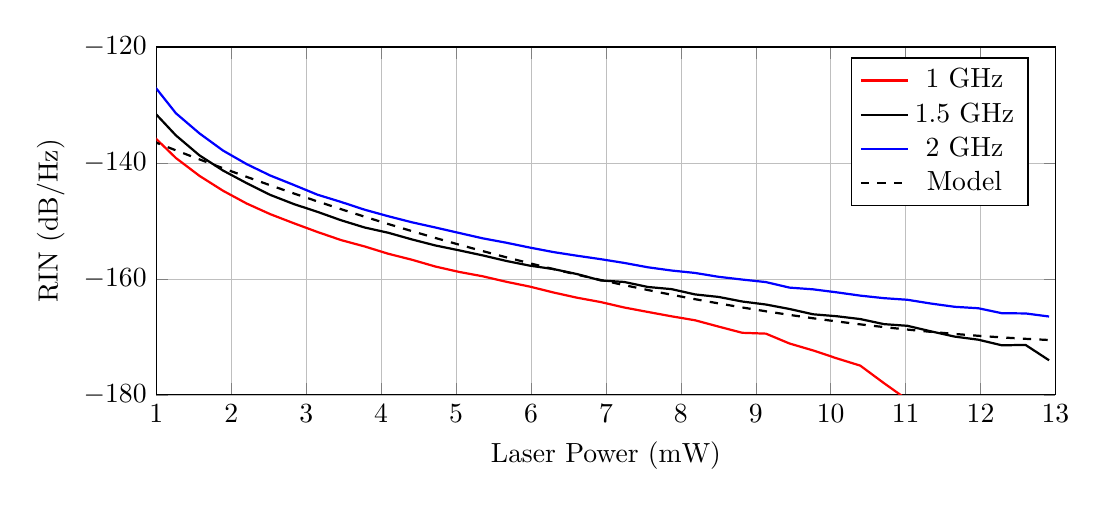
\begin{tikzpicture}
\begin{axis}[width={13cm}, height={6cm}, grid={both}, grid style={line width={.1pt}, draw={gray!10}}, major grid style={line width={.2pt}, draw={gray!50}}, legend pos={north east}, xlabel={Laser Power (mW)}, ylabel={RIN (dB/Hz)},xmin=1,xmax=13,ymin=-180,ymax=-120]
    \addplot[no marks, thick, color={red}]
        coordinates {
            (0.9449999999999997,-135.20023466155118)
            (1.26,-139.14586462255016)
            (1.5750000000000002,-142.22930277186612)
            (1.89,-144.80197811803637)
            (2.205,-146.9995585469889)
            (2.52,-148.83731640984507)
            (2.8350000000000004,-150.4055285897713)
            (3.1500000000000004,-151.91089960473383)
            (3.465,-153.30737321536665)
            (3.78,-154.40753328456435)
            (4.095000000000001,-155.66577937061612)
            (4.41,-156.69538147511457)
            (4.725,-157.87336569921354)
            (5.04,-158.79665884505505)
            (5.355,-159.54993257463354)
            (5.670000000000001,-160.49755044018409)
            (5.984999999999999,-161.3329805733184)
            (6.3,-162.34601163588525)
            (6.615,-163.2473387881319)
            (6.93,-163.9947659502225)
            (7.245,-164.93599985033546)
            (7.56,-165.70263004791184)
            (7.875,-166.45197413630456)
            (8.190000000000001,-167.13743105344315)
            (8.505,-168.23170909489795)
            (8.820000000000002,-169.29832572341766)
            (9.135,-169.44202824608152)
            (9.45,-171.1435279323556)
            (9.764999999999999,-172.33887562560915)
            (10.08,-173.69840913574365)
            (10.395,-174.9597405818915)
            (10.71,-177.9719995442211)
            (11.025000000000002,-180.860535423638)
            (11.34,-186.3206846748801)





        }
        ;
    \addlegendentry {1 GHz}
    \addplot[no marks, thick, color={black}]
        coordinates {
            (0.9449999999999997,-130.9038379538291)
            (1.26,-135.24456274600675)
            (1.5750000000000002,-138.6983670608943)
            (1.89,-141.31582281469431)
            (2.205,-143.487239180235)
            (2.52,-145.5133242116656)
            (2.8350000000000004,-147.09573475252515)
            (3.1500000000000004,-148.4373676189136)
            (3.465,-149.8883105516857)
            (3.78,-151.13884529733636)
            (4.095000000000001,-152.04423199057481)
            (4.41,-153.19225371839542)
            (4.725,-154.23942241565078)
            (5.04,-155.07389862856886)
            (5.355,-155.947633873557)
            (5.670000000000001,-156.9046547127191)
            (5.984999999999999,-157.72003512737595)
            (6.3,-158.30471314174272)
            (6.615,-159.17037299575375)
            (6.93,-160.2651514248512)
            (7.245,-160.53093960621052)
            (7.56,-161.3945245486463)
            (7.875,-161.76301572588343)
            (8.190000000000001,-162.67884618167898)
            (8.505,-163.1141329423886)
            (8.820000000000002,-163.9035207536444)
            (9.135,-164.41874248698957)
            (9.45,-165.18955931155116)
            (9.764999999999999,-166.10523695664915)
            (10.08,-166.43926463622313)
            (10.395,-166.92766794192235)
            (10.71,-167.80070381544675)
            (11.025000000000002,-168.09362014610468)
            (11.34,-169.05409490650362)
            (11.655,-169.95439011786095)
            (11.969999999999999,-170.48643782925024)
            (12.285,-171.45678587360584)
            (12.6,-171.3831140779719)
            (12.915000000000001,-174.04084511894223)
        }
        ;
    \addlegendentry {1.5 GHz}
    \addplot[no marks, thick, color={blue}]
        coordinates {
            (0.9449999999999997,-126.28216502258195)
            (1.26,-131.4263968893813)
            (1.5750000000000002,-134.90502733972454)
            (1.89,-137.87073346498227)
            (2.205,-140.20498383730765)
            (2.52,-142.17271970902254)
            (2.8350000000000004,-143.80489140376253)
            (3.1500000000000004,-145.4781719695783)
            (3.465,-146.7316159443491)
            (3.78,-148.0696801255849)
            (4.095000000000001,-149.19368781834902)
            (4.41,-150.23615603895794)
            (4.725,-151.14090710598563)
            (5.04,-152.0758159264305)
            (5.355,-153.0044044452289)
            (5.670000000000001,-153.76175983613234)
            (5.984999999999999,-154.60173252946498)
            (6.3,-155.37703376055737)
            (6.615,-156.00631840742568)
            (6.93,-156.59771087110758)
            (7.245,-157.24824033587677)
            (7.56,-157.99899073852018)
            (7.875,-158.55545275915574)
            (8.190000000000001,-158.97592516356164)
            (8.505,-159.64244151615515)
            (8.820000000000002,-160.117098225336)
            (9.135,-160.55145085072866)
            (9.45,-161.50357222094334)
            (9.764999999999999,-161.80185417537058)
            (10.08,-162.3183159255533)
            (10.395,-162.88661148733274)
            (10.71,-163.32222993473238)
            (11.025000000000002,-163.60453245214316)
            (11.34,-164.2560796511731)
            (11.655,-164.81465471913447)
            (11.969999999999999,-165.06163129756243)
            (12.285,-165.92023515514944)
            (12.6,-165.9572471757354)
            (12.915000000000001,-166.48900184048108)
        }
        ;
    \addlegendentry {2 GHz}
    \addplot[no marks, thick, color={black}, dashed]
        coordinates {
            (0.9449999999999997,-136.22782524999997)
            (1.26,-137.82835599999999)
            (1.5750000000000002,-139.39118125)
            (1.89,-140.916301)
            (2.205,-142.40371524999998)
            (2.52,-143.853424)
            (2.8350000000000004,-145.26542725)
            (3.1500000000000004,-146.63972499999997)
            (3.465,-147.97631725)
            (3.78,-149.27520399999997)
            (4.095000000000001,-150.53638525)
            (4.41,-151.75986099999997)
            (4.725,-152.94563125)
            (5.04,-154.093696)
            (5.355,-155.20405524999998)
            (5.670000000000001,-156.27670899999998)
            (5.984999999999999,-157.31165724999997)
            (6.3,-158.3089)
            (6.615,-159.26843724999998)
            (6.93,-160.190269)
            (7.245,-161.07439524999998)
            (7.56,-161.92081599999997)
            (7.875,-162.72953124999998)
            (8.190000000000001,-163.500541)
            (8.505,-164.23384525)
            (8.820000000000002,-164.929444)
            (9.135,-165.58733725)
            (9.45,-166.20752499999998)
            (9.764999999999999,-166.79000724999997)
            (10.08,-167.33478399999998)
            (10.395,-167.84185525)
            (10.71,-168.311221)
            (11.025000000000002,-168.74288124999998)
            (11.34,-169.136836)
            (11.655,-169.49308524999998)
            (11.969999999999999,-169.81162899999998)
            (12.285,-170.09246724999997)
            (12.6,-170.3356)
            (12.915000000000001,-170.54102724999998)
        }
        ;
    \addlegendentry {Model}
\end{axis}
\end{tikzpicture}
\end{document}